\documentclass{article}

\usepackage{ngerman}
\usepackage[T1]{fontenc}
\usepackage[utf8]{inputenc}
\usepackage{graphicx}			% Moderne Grafikeinbinung
\usepackage{lmodern}			% schöne flüssige schrift

\usepackage{tikz}
\usetikzlibrary{calc}

\begin{document}
\centering
\scalebox{-1}[1]{
\begin{tikzpicture}[x=10cm,y=7cm]

\fill [white] (0,0) rectangle (1,1);

\def\padhight{.15}
\def\mid{\padhight}
\def\top{\mid+\padhight}

\def\solderspace{.5-\padhight}
\def\topp{\top+\solderspace}
\def\toppp{\topp+\solderspace}

\draw[white] (0,\mid) -- (1,\mid);

\def\interval{1/7}
\def\offset{1/14}
\def\frameh{.015}
\def\framev{.01}

\Large

\foreach \x in {0,1,2,3,4,5,6}
	{
	\def\centerx{\offset+\x*\interval}
	\def\centery{\padhight/2}
	\fill[black] (\centerx-\offset+\framev,\centery-\padhight/2+\frameh) rectangle (\centerx+\offset-\framev,\centery+\padhight/2-\frameh);
		
	% B2 D3 F3 A3 C4 E4 G4
	\ifcase\x
		\def\notetext{B$_2$}
	\or
		\def\notetext{D$_3$}
	\or
		\def\notetext{F$_3$}
	\or
		\def\notetext{A$_3$}
	\or
		\def\notetext{C$_4$}
	\or
		\def\notetext{E$_4$}
	\or
		\def\notetext{G$_4$}
	\fi	
	
	\node[text=white] at (\centerx,\centery) {\textbf{\notetext}};
	}

\def\interval{.96/6}
\def\offset{1/12+.01}
\def\frameh{.01}
\def\framev{.03}

\foreach \x in {0,1,2,3,4,5}
	{
	\def\offset{1/12+.01}
	\def\centerx{\offset+\x*\interval}
	\def\centery{3*\padhight/2}
	\fill[black] (\centerx-\offset+\framev,\centery-\padhight/2+\frameh) rectangle (\centerx+\offset-\framev,\centery+\padhight/2-\frameh);
	\def\offset{1/12+.02}
	
	% C3 E3 G3 B3 D4 F4
	\ifcase\x
		\def\notetext{C$_3$}
	\or
		\def\notetext{E$_3$}
	\or
		\def\notetext{G$_3$}
	\or
		\def\notetext{B$_3$}
	\or
		\def\notetext{D$_4$}
	\or
		\def\notetext{F$_4$}
	\fi	
	
	\node[text=white] at (\centerx,\centery) {\textbf{\notetext}};
	}

\def\interval{1/13}
\def\offset{1/26}
\def\frameh{.04}
\def\framev{.01}
\def\padhight{.15}
\def\solpad{.35}

\foreach \x in {0,1,2,3,4,5,6,7,8,9,10,11,12}
	{
	\def\centerx{\offset+\x*\interval}
	\def\centery{\solpad}
	\fill[black] (\centerx-\offset+\framev,\centery-\padhight/2+\frameh) rectangle (\centerx+\offset-\framev,\centery+\padhight/2-\frameh);
	}

\def\interval{1/6.34}
\def\offset{.03}
\def\lowend{.13}
\foreach \x in {0,1,2,3,4,5,6}
	{
	\draw[black,line width=0.15cm] (\x*\interval+\offset,\lowend) -- (\x*\interval+\offset,\solpad);
	}

\def\offset{.106}
\def\lowend{.29}
\foreach \x in {0,1,2,3,4,5}
	{
	\draw[black,line width=0.15cm] (\x*\interval+\offset,\lowend) -- (\x*\interval+\offset,\solpad);
	}

\fill[black] (0+\framev,1-\framev) rectangle (1-\framev,.405);
%\fill [red] (0,1) rectangle (.3,1-2/7);
%\fill [green] (1,1) rectangle (.5,1-2.7/7);

\coordinate (D) at (.195,.845);
\coordinate (E) at (.19,.155);
\fill [white] ($ (D) - (E) $) rectangle ($ (D) + (E) $);
\node at ($ (D) + (0,.1245) $) {
%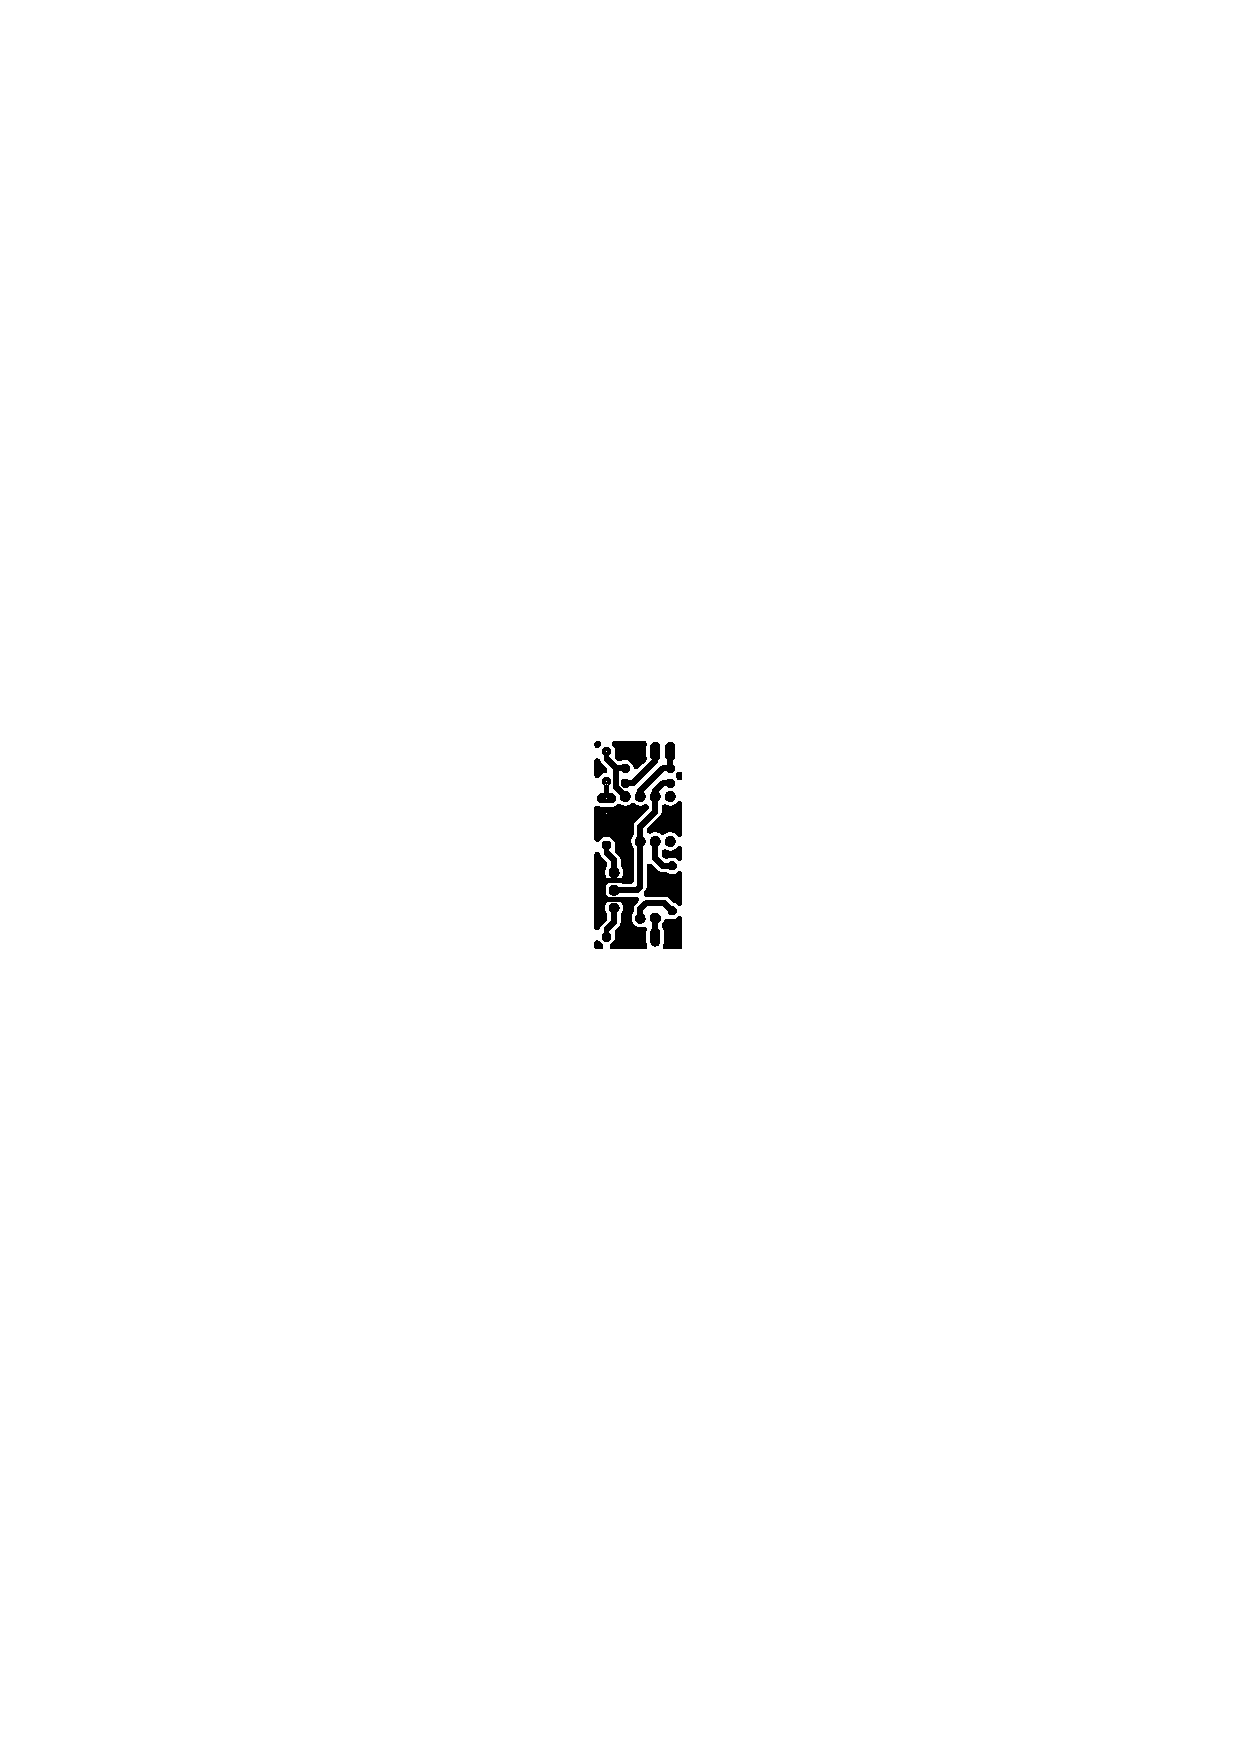
\includegraphics[angle=-90]{circuite}
%				 trim=left bottom right top
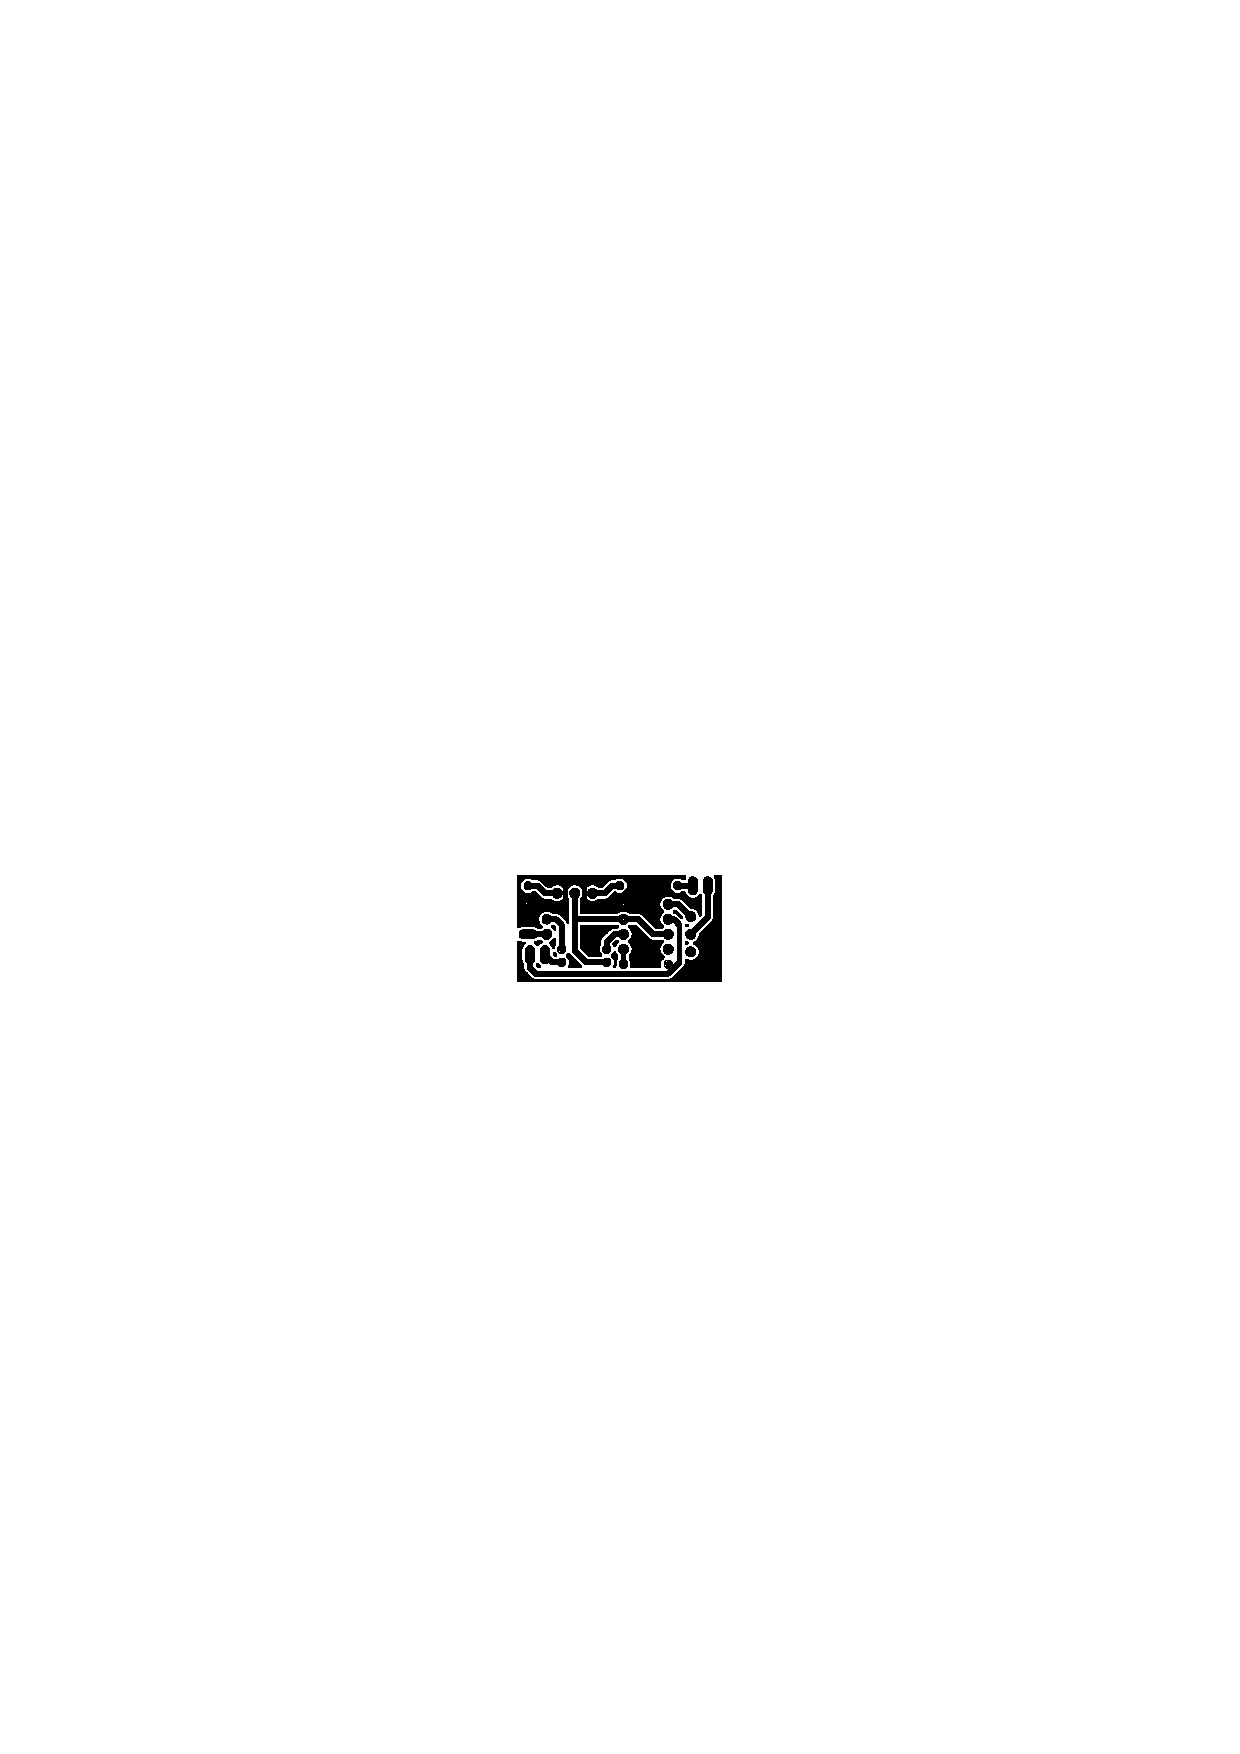
\includegraphics[trim=7cm 13cm 7cm 13cm, clip]{555piano}
};

\draw [black] (0,0) rectangle (1,1); 

\end{tikzpicture}
}
\end{document}